% This is "sig-alternate.tex" V2.1 April 2013
% This file should be compiled with V2.5 of "sig-alternate.cls" May 2012
%
% This example file demonstrates the use of the 'sig-alternate.cls'
% V2.5 LaTeX2e document class file. It is for those submitting
% articles to ACM Conference Proceedings WHO DO NOT WISH TO
% STRICTLY ADHERE TO THE SIGS (PUBS-BOARD-ENDORSED) STYLE.
% The 'sig-alternate.cls' file will produce a similar-looking,
% albeit, 'tighter' paper resulting in, invariably, fewer pages.
%
% ----------------------------------------------------------------------------------------------------------------
% This .tex file (and associated .cls V2.5) produces:
%       1) The Permission Statement
%       2) The Conference (location) Info information
%       3) The Copyright Line with ACM data
%       4) NO page numbers
%
% as against the acm_proc_article-sp.cls file which
% DOES NOT produce 1) thru' 3) above.
%
% Using 'sig-alternate.cls' you have control, however, from within
% the source .tex file, over both the CopyrightYear
% (defaulted to 200X) and the ACM Copyright Data
% (defaulted to X-XXXXX-XX-X/XX/XX).
% e.g.
% \CopyrightYear{2007} will cause 2007 to appear in the copyright line.
% \crdata{0-12345-67-8/90/12} will cause 0-12345-67-8/90/12 to appear in the copyright line.
%
% ---------------------------------------------------------------------------------------------------------------
% This .tex source is an example which *does* use
% the .bib file (from which the .bbl file % is produced).
% REMEMBER HOWEVER: After having produced the .bbl file,
% and prior to final submission, you *NEED* to 'insert'
% your .bbl file into your source .tex file so as to provide
% ONE 'self-contained' source file.
%
% ================= IF YOU HAVE QUESTIONS =======================
% Questions regarding the SIGS styles, SIGS policies and
% procedures, Conferences etc. should be sent to
% Adrienne Griscti (griscti@acm.org)
%
% Technical questions _only_ to
% Gerald Murray (murray@hq.acm.org)
% ===============================================================
%
% For tracking purposes - this is V2.0 - May 2012

\documentclass{sig-alternate-05-2015}

\usepackage[square,numbers]{natbib}
\usepackage[justification=centering]{caption}
\usepackage[pageanchor=true,plainpages=false,pdfpagelabels,bookmarks,bookmarksnumbered,hidelinks]{hyperref}
\usepackage{color}
\definecolor{mygray}{rgb}{0.6,0.6,0.6}
\definecolor{lightgray}{rgb}{0.92,0.92,0.92}
\definecolor{darkgreen}{rgb}{0,0.7,0}

% for footnotes in tables
\usepackage{tablefootnote}

% for title caps
\usepackage{titlecaps}
\Addlcwords{and, the, or, of, that, our, by, a, prevent, for}

% default options for listings
\usepackage{listings}
\usepackage{listingsutf8}
\usepackage{textcomp}     % access \textquotesingle
\lstset{
	backgroundcolor=\color{lightgray},
	basicstyle=\footnotesize,
	breaklines=true, 
	captionpos=b,
	commentstyle=\color{darkgreen}, 
	frame=single,
	keywordstyle=\color{blue}, 
	numbers=left,
	numbersep=5pt,
	numberstyle=\tiny\color{mygray},
	rulecolor=\color{black},
	showstringspaces=false,
	upquote=true
}

	
\newcommand{\dq}[1]{``{#1}''}
%% THIS IS THE DATA FOR OUR THESIS, UPDATING HERE WILL UPDATE EVERYWHERE %%
\newcommand{\urls}{21,675,680}

\newcommand{\forms}{6,794,917}
\newcommand{\formsDelta}{31.35\%}

\newcommand{\emailforms}{1,132,157}
\newcommand{\emailformsDelta}{16.66\%}

\newcommand{\fuzzed}{934,016}
\newcommand{\fuzzedDelta}{82.50\%}

\newcommand{\recd}{52,724}
\newcommand{\recdDelta}{5.64\%}

\newcommand{\malfuzzed}{46,156}
\newcommand{\malfuzzedDelta}{87.54\%}

\newcommand{\success}{496}
\newcommand{\successDelta}{1.07\%}

\newcommand{\domains}{222}
\newcommand{\ips}{292}
% these refer to unique domains, not unique forms
\newcommand{\uniqueforms}{1,019,921}
\newcommand{\uniqueemailforms}{197,570}


\begin{document}
	
	% Copyright
	\setcopyright{acmcopyright}
	%\setcopyright{acmlicensed}
	%\setcopyright{rightsretained}
	%\setcopyright{usgov}
	%\setcopyright{usgovmixed}
	%\setcopyright{cagov}
	%\setcopyright{cagovmixed}
	
	
	% DOI
	\doi{10.475/123_4}
	
	% ISBN
	\isbn{123-4567-24-567/08/06}
	
	%Conference
	\conferenceinfo{PLDI '13}{June 16--19, 2013, Seattle, WA, USA}
	
	\acmPrice{\$15.00}
	
	%
	% --- Author Metadata here ---
	\conferenceinfo{WOODSTOCK}{'97 El Paso, Texas USA}
	%\CopyrightYear{2007} % Allows default copyright year (20XX) to be over-ridden - IF NEED BE.
	%\crdata{0-12345-67-8/90/01}  % Allows default copyright data (0-89791-88-6/97/05) to be over-ridden - IF NEED BE.
	% --- End of Author Metadata ---
	
	\title{E-jection fraction - Tracking how your website pumps out E-Mails}
	%
	% You need the command \numberofauthors to handle the 'placement
	% and alignment' of the authors beneath the title.
	%
	% For aesthetic reasons, we recommend 'three authors at a time'
	% i.e. three 'name/affiliation blocks' be placed beneath the title.
	%
	% NOTE: You are NOT restricted in how many 'rows' of
	% "name/affiliations" may appear. We just ask that you restrict
	% the number of 'columns' to three.
	%
	% Because of the available 'opening page real-estate'
	% we ask you to refrain from putting more than six authors
	% (two rows with three columns) beneath the article title.
	% More than six makes the first-page appear very cluttered indeed.
	%
	% Use the \alignauthor commands to handle the names
	% and affiliations for an 'aesthetic maximum' of six authors.
	% Add names, affiliations, addresses for
	% the seventh etc. author(s) as the argument for the
	% \additionalauthors command.
	% These 'additional authors' will be output/set for you
	% without further effort on your part as the last section in
	% the body of your article BEFORE References or any Appendices.
	
	\numberofauthors{8} %  in this sample file, there are a *total*
	% of EIGHT authors. SIX appear on the 'first-page' (for formatting
	% reasons) and the remaining two appear in the \additionalauthors section.
	%
	\author{
		% You can go ahead and credit any number of authors here,
		% e.g. one 'row of three' or two rows (consisting of one row of three
		% and a second row of one, two or three).
		%
		% The command \alignauthor (no curly braces needed) should
		% precede each author name, affiliation/snail-mail address and
		% e-mail address. Additionally, tag each line of
		% affiliation/address with \affaddr, and tag the
		% e-mail address with \email.
		%
		% 1st. author
		\alignauthor
		Ben Trovato\titlenote{Dr.~Trovato insisted his name be first.}\\
		\affaddr{Institute for Clarity in Documentation}\\
		\affaddr{1932 Wallamaloo Lane}\\
		\affaddr{Wallamaloo, New Zealand}\\
		\email{trovato@corporation.com}
		% 2nd. author
		\alignauthor
		G.K.M. Tobin\titlenote{The secretary disavows
			any knowledge of this author's actions.}\\
		\affaddr{Institute for Clarity in Documentation}\\
		\affaddr{P.O. Box 1212}\\
		\affaddr{Dublin, Ohio 43017-6221}\\
		\email{webmaster@marysville-ohio.com}
		% 3rd. author
		\alignauthor Lars Th{\o}rv{\"a}ld\titlenote{This author is the
			one who did all the really hard work.}\\
		\affaddr{The Th{\o}rv{\"a}ld Group}\\
		\affaddr{1 Th{\o}rv{\"a}ld Circle}\\
		\affaddr{Hekla, Iceland}\\
		\email{larst@affiliation.org}
		\and  % use '\and' if you need 'another row' of author names
		% 4th. author
		\alignauthor Lawrence P. Leipuner\\
		\affaddr{Brookhaven Laboratories}\\
		\affaddr{Brookhaven National Lab}\\
		\affaddr{P.O. Box 5000}\\
		\email{lleipuner@researchlabs.org}
		% 5th. author
		\alignauthor Sean Fogarty\\
		\affaddr{NASA Ames Research Center}\\
		\affaddr{Moffett Field}\\
		\affaddr{California 94035}\\
		\email{fogartys@amesres.org}
		% 6th. author
		\alignauthor Charles Palmer\\
		\affaddr{Palmer Research Laboratories}\\
		\affaddr{8600 Datapoint Drive}\\
		\affaddr{San Antonio, Texas 78229}\\
		\email{cpalmer@prl.com}
	}
	% There's nothing stopping you putting the seventh, eighth, etc.
	% author on the opening page (as the 'third row') but we ask,
	% for aesthetic reasons that you place these 'additional authors'
	% in the \additional authors block, viz.
	\additionalauthors{Additional authors: John Smith (The Th{\o}rv{\"a}ld Group,
		email: {\texttt{jsmith@affiliation.org}}) and Julius P.~Kumquat
		(The Kumquat Consortium, email: {\texttt{jpkumquat@consortium.net}}).}
	\date{30 July 1999}
	% Just remember to make sure that the TOTAL number of authors
	% is the number that will appear on the first page PLUS the
	% number that will appear in the \additionalauthors section.
	
	\maketitle
	\begin{abstract}
	\ehi vulnerability is a class of vulnerability that can occur in web applications that use user input to construct \email messages. \ehi is possible when the mailing script fails to check for the presence of \email headers in user input (either form fields or URL parameters). The vulnerability exists in the reference implementation of the built-in mail functionality in popular languages such as PHP, Java, Python, and Ruby. With the proper injection string, this vulnerability can be exploited to inject additional headers, modify existing headers, and  alter the content of the \email.
	
	This paper presents a scalable mechanism to automatically detect \ehi vulnerabilities and uses this mechanism to quantify the prevalence of \ehi vulnerabilities on the web. Using a black-box testing approach, the system crawled \urls URLs identify web pages which contained form fields. \forms such forms were found by the system, of which \emailforms forms contained \email fields. We then tested \fuzzed forms to see if they would send us an \email, and \recd forms sent us an \email. Of these \malfuzzed forms were tested with \ehi payloads and, of these, we found \success vulnerable URLs across \domains domains. Then, to demonstrate that \ehi vulnerabilities are actively being exploited to create a spamming platform, we found \ipsblacklist IPs that were vulnerable on well-known spamming blacklists. This work shows that \ehi vulnerabilities are widespread and deserve future research attention.
\end{abstract}

	
	
	%
	% The code below should be generated by the tool at
	% http://dl.acm.org/ccs.cfm
	% Please copy and paste the code instead of the example below. 
	%
	\begin{CCSXML}
		<ccs2012>
		<concept>
		<concept_id>10010520.10010553.10010562</concept_id>
		<concept_desc>Computer systems organization~Embedded systems</concept_desc>
		<concept_significance>500</concept_significance>
		</concept>
		<concept>
		<concept_id>10010520.10010575.10010755</concept_id>
		<concept_desc>Computer systems organization~Redundancy</concept_desc>
		<concept_significance>300</concept_significance>
		</concept>
		<concept>
		<concept_id>10010520.10010553.10010554</concept_id>
		<concept_desc>Computer systems organization~Robotics</concept_desc>
		<concept_significance>100</concept_significance>
		</concept>
		<concept>
		<concept_id>10003033.10003083.10003095</concept_id>
		<concept_desc>Networks~Network reliability</concept_desc>
		<concept_significance>100</concept_significance>
		</concept>
		</ccs2012>  
	\end{CCSXML}
	
	\ccsdesc[500]{Computer systems organization~Embedded systems}
	\ccsdesc[300]{Computer systems organization~Redundancy}
	\ccsdesc{Computer systems organization~Robotics}
	\ccsdesc[100]{Networks~Network reliability}
	
	
	%
	% End generated code
	%
	
	%
	%  Use this command to print the description
	%
	\printccsdesc
	
	% We no longer use \terms command
	%\terms{Theory}
	
	\keywords{ACM proceedings; \LaTeX; text tagging}

	\section{Introduction}
The World Wide Web has single-handedly brought about a change in the way we use computers. The ubiquitous nature of the web has made it possible for anyone to access information and services anywhere and on multiple devices such as phones, laptops, personal digital assistants, TVs, and cars. This access has ushered in an era of web applications which depend on user input. While this rapid pace of development has improved the speed of dissemination of information, it does come at a cost. As users move more and more of their personal and financial information to web applications, attackers are responding by using web application vulnerabilities to access this lucrative data.

%% Adam: I don't see how this adds to our story
%% Attackers have an added incentive to break into user's e-mail accounts more than ever. E-Mail accounts are usually connected to almost all other online accounts of a user, and e-mails continue to serve as the principal mode of official communication on the web for most institutions. Thus, the impact an attacker can have by having control over the \email communication sent by websites to users is of an enormous magnitude.

% TODO: Sai, can you add a reference to command injection vulnerabilities here? DONE.
Many common and well-known web application vulnerabilities, such as SQL Injection and Cross-Site Scripting~\cite{OWASPT10}, are command injection vulnerabilities~\cite{commandinjection}, where malicious user input is used to alter the structure of a command (a SQL query in the case of SQL Injection and JavaScript code in the case of Cross-Site Scripting). Developers of web applications must have proper sanitization routines in place to use user input as part of these commands. 

\ehi vulnerabilities are a lesser-known command injection vulnerability. \ehi can be considered as the \email equivalent of HTTP Header Injection~\cite{wiki:HTTP_headerinjection}. This vulnerability exists in the implementation of the built-in \texttt{mail} functionality in popular languages such as PHP, Java, Python, and Ruby. The format of \email messages is defined by the Simple Mail Transfer Protocol (SMTP)~\cite{rfc5322}. Each \email message is represented by a series of headers separated by newlines, followed by the body content (separated from the headers by two newlines). Some of these headers are mandatory (From, To, Date), but the headers could also include other information like the Subject, CC, BCC, etc.

%\textbf{Sai: I believe that the discussion of SMTP Headers belongs here, before we say that E-Mail Header Injection can manipulate the headers. Do I need to include the message format as a listing? I think its superfluous, but let me know.}

With the proper injection string, \ehi vulnerabilities can be exploited by an attacker to inject additional headers, modify existing headers, or alter the contents of the \email---while still appearing to be from a legitimate source. \ehi exploits allow an attacker to perform \email spoofing, resulting in phishing attacks \emph{that are sent from the actual \email server}.

%% The objective of our research is to study the prevalence of this vulnerability on the World Wide Web, and identify whether further research is required in this area.

While some command injection vulnerabilities have received extensive attention from the research community, \ehi vulnerabilities have received little focus. Therefore, we study the prevalence of \ehi vulnerabilities on the web. We performed a crawl of the web, extracted forms with \email fields, and injected them with different payloads to infer the existence of an \ehi vulnerability. We then audited received \emails to see if any of the injected data was present. This allowed us to classify whether a particular URL was vulnerable to the attack. Our automated system works in a black-box manner, without looking at the web application's source code, and only analyzes the \emails we receive based on the injected payloads.
\\

\noindent{}In summary, we make the following contributions:

\begin{itemize}

\item We develop a black-box approach to detect \ehi vulnerabilities in a web application.

\item We develop a system to crawl the web and automatically detect \ehi vulnerabilities.

\item We use our system to crawl \urls URLs, and we find \success URLs vulnerable to \ehi across \domains domains. 

\end{itemize}

	
	\section{Background}
\section{Problem Background}

E-Mail Header Injection belongs to a broad class of vulnerabilities known simply as injection attacks. However, unlike its more popular siblings, SQL injection \cite{sql1}, \cite{sql0}, \cite{sql2}, Cross-Site Scripting (XSS) \cite{Injection1}, \cite{KleinAmit} or even HTTP Header Injection \cite{sessionride}, relatively little research is available on E-Mail Header Injection.

As with other vulnerabilities in this class, E-Mail Header Injection is caused due to improper sanitization (or lack thereof) of user input. If the script that constructs e-mails from user input fails to check for the presence of e-mail headers in the user input, a malicious user --- using a well-crafted payload --- can control the headers set for this particular e-mail. This can be leveraged to enable malicious attacks, including, but not limited to, spoofing, phishing, etc.
\subsection{History of \ehi}

We found the first \ehi description in a late 2004 article on phpsecure.info~\cite{Tobozo} accredited to user \lstinline|tobozo@phpsecure.info| describing how an \ehi vulnerability existed in the implementation of the \texttt{mail()} function in PHP and how it can be exploited. More recently, a blog post by Damon Kohler~\cite{DK} and an accompanying wiki article~\cite{Injection} describe the attack vector and outline few defense measures for \ehi vulnerabilities.

%% As this vulnerability was initially found in the \texttt{mail()} function of PHP, \ehi can be traced to as early as the beginning of the 2000's, present in the \texttt{mail()} implementation of PHP 4.0. 

An example of the vulnerable code written in PHP is shown in Listing~\ref{code:phpemi}. This code takes in user input from the PHP superglobal \texttt{\$\_REQUEST[\textquotesingle email\textquotesingle]}, and stores it in the variable \texttt{\$from}, which is later passed to the \texttt{mail()} function to construct and send the e-mail.

\begin{lstlisting}[language=PHP,caption={PHP program with e-mail
      header injection vulnerability.},label={code:phpemi}, float]
$from = $_REQUEST['email'];
$subject = 'Hello XYZ';
$message = 'We need you to reset your password';
$to = 'xyz@example.com';
$retValue = mail($to, $subject, $message, "From: $from");
\end{lstlisting}



% TODO: Change all domains to example.com
% TODO: Sai, this is the first time we mention SMTP, need more background and a reference to the RFC.

\textbf{Adam: This example is not correct, the STMP headers in listing 2 should have the "From" headers from the injection.}

When this code is given the malicious input \texttt{\lstinline{sai@sai.com\\nCC:spc@spc.com}} as the value of the \texttt{\$\_REQUEST[\textquotesingle email\textquotesingle]}, it generates the SMTP Headers shown in Listing~\ref{code:smtpheaders}. It can be seen that the \texttt{CC} (carbon copy) header that we injected appears as part of the resulting SMTP message. This will make the e-mail get sent to the e-mail address specified as part of the \texttt{CC} as well. 
\begin{lstlisting}[language=HTML,caption={SMTP headers generated by a PHP mailing
  script.},label={code:smtpheaders}, float]
Received: from mail.ourdomain.com ([62.121.130.29])
  by xyz.com (Postfix) with ESMTP id 5A08E52C0154
  for <abc@example.com>; Sun, 20 Mar 2016 13:56:58 -0700 (MST)
From: abc@example.com
To: xyz@example.com
Subject: Hello XYZ
CC: spc@example.com
Date: Sun, 20 Mar 2016 13:56:58 -0700 (MST)

We need you to reset your password
\end{lstlisting}

%\begin{table}[!htbp]
	\centering
	\begin{tabular}{|p{2cm}|p{12cm}|}
		\hline
		\multicolumn{1}{|c|}{\textbf{Year}} & \multicolumn{1}{c|}{\textbf{ Notes}}\\
		\hline

		{Early 2000's } & { PHP 4.0 is released, along with support for the mail() function, which has no protection against E-Mail Header Injection.}\\
		\hline

		{Jul 2004} & { Next Major version of PHP - Version 5.0 releases}\\
		\hline

		{Dec 2004} & { First known article about the vulnerability surfaces on phpsecure.info}\\
		\hline

		{Oct 2007} & {The vulnerability makes its way into a text by Stuttard and Pinto. }\\
		\hline

		{Dec 2008} & {Blog post and accompanying wiki about the header injection attack in detail with examples.}\\
		\hline

		{Apr 2009} & {Bug filed about email.header package to fix the issue on Python Bug Tracker}\\
		\hline

		{Jan 2011} & {Bug fix for Python 3.1, Python 3.2, Python 2.7 for email.header package, backport to older versions not available.}\\
		\hline

		{Sep 2011} & {The vulnerability is described with an example in the 2nd edition of the text by Stuttard and Pinto.}\\
		\hline

		{Aug 2013} & {Acunetix adds E-Mail Header Injection to the list of vulnerabilties they detect, as part of their Enterprise Web Vulnerability Scanner Software.}\\
		\hline

		{May 2014} & {Security Advisory for JavaMail SMTP Header Injection via method setSubject is written by Alexandre Herzog.}\\
		\hline

		{Dec 2015}  & {PHP 7 releases, mail function still unpatched.}\\
		\hline
	\end{tabular}
	\caption[\titlecap{A brief history of e-mail header injection}]{A brief history of e-mail header injection.}
	\label{tab:history}
\end{table}


\subsection{Languages Affected}
\label{languages}
\noindent{\textbf{PHP}} was the first language found vulnerable to \ehi in its implementation of the \texttt{mail()} function at the time of release of PHP~4.0. According to w3techs~\cite{W3techs}, PHP is used by 81.9\% of all websites.

After 13 further iterations of PHP since the 4.0 release (the current
version is 7.1), the \texttt{mail()} function is yet to be fixed after
15 years. However, the PHP documentation~\cite{PHPDocs} specifies that the \texttt{mail()} function does not protect against \ehi.
A working code sample with the vulnerability is shown in  Listing~\ref{code:phpemi}.

\begin{sloppypar}
A bug was filed about an \ehi vulnerability in Python's implementation of the \texttt{email.header} library and the header parsing functions allowing newlines in early 2009, which was followed by a partial patch in 2011.
\end{sloppypar}

Unfortunately, the bug fix was only for the \texttt{email.header} package, and not for other frequently used packages such as \texttt{email.parser}, where both the classic \texttt{Parser()} and the newer \texttt{FeedParser()} contain \ehi vulnerabilities even in the latest versions: \texttt{2.7.11} and \texttt{3.5}. The bug fix was also not backported to older versions of Python.
There is no mention of the vulnerability in the Python documentation for either library. Contrary to PHP's behavior of overwriting existing headers, Python only recognizes the first occurrence of a header, and ignores duplicate headers.

%A working code sample of the vulnerability, written in Python 2.7.11, is shown in Listing~\ref{code:pyemi}.

%\begin{lstlisting}[language=Python,caption={Python program with e-mail
      header injection vulnerability.},label={code:pyemi}, float]
from email.parser import Parser
import cgi
form = cgi.FieldStorage()
to = form["email"] # input() exhibits 
# the same behavior
msg = """To: """ + to + """\n
From: <user@example.com>\n
Subject: Test message\n\n
Body would go here\n"""

f = FeedParser() # Parser.parsestr() 
# also contains the same vulnerability
f.feed(msg)
headers = FeedParser.close(f)

# attack string => 
# 'abc@example.com\nBCC:spc@example.com'
# for form["email"]

# to:abc@example.com AND bcc:spc@example.com 
# are added to the headers
print 'To: %s' % headers['to']
print 'BCC: %s' % headers['bcc']
\end{lstlisting}


Java has a bug report about \ehi filed against its \texttt{JavaMail} API. A detailed write-up by Alexandre Herzog~\cite{Herzog.2014} contains a proof-of-concept program that exploits the API to inject headers.

\begin{sloppypar}
From our preliminary testing, Ruby's built-in \texttt{Net::SMTP} library also has an \ehi vulnerability (not documented on the library's homepage).
%A working code sample of the vulnerability, written in Ruby 2.0.0 (the latest stable version at the time of writing), is shown in Listing~\ref{code:rubyemi}.
\end{sloppypar}
%\begin{lstlisting}[language=Ruby,caption={Ruby program with e-mail
      header injection vulnerability.},label={code:rubyemi}, float]
require 'sinatra'
require 'net/smtp'

get '/hello' do
email = params[:email]

message = """
From: Sai <schand31@asu.edu>
Subject: SMTP e-mail test
To: #{email}

This is a test e-mail message.
"""
# construct a post request with email set to attack_string
# attack_string => sai@sai.com%0abcc:spc@spc.com%0aSubject:Hello
Net::SMTP.start('localhost', 1025) do |smtp|
smtp.send_message message, 'schand31@asu.edu',
'to@todomain.com'
end
# Headers get added, and Subject field changes to what we set.
end
\end{lstlisting}




\subsection{Exploitation}
\label{exploitation}
Successful exploitation of an \ehi vulnerability depends on where
injection occurs in the SMTP message. The attacker cannot alter parts
of the SMTP message that precede the injection location, but the
attacker has complete control over everything that follows. However,
similar to other command injection vulnerabilities, the remaining
parts of the SMTP message will always be appended to the attacker's
injection, so the attacker must contend with this. By
exploiting an \ehi vulnerability, an attacker can control who receives
the message (and can include multiple \texttt{CC} and \texttt{BCC}
recipients), the body, and possibly the subject (depending on if the subject header occurs
before/after the injection point and the language used).

\begin{lstlisting}[language=HTML,caption={Exploiting the \ehi
      vulnerability in Listing~\ref{code:phpemi} to control the
      recipients, subject, and body of the SMTP message.},label={code:ehiexploit}, float]
Received: from mail.ourdomain.com ([62.121.130.29])
  by xyz.com (Postfix) with ESMTP id 5A08E52C0154
  for <abc@example.com>; Sun, 20 Mar 2016 13:56:58 -0700 (MST)
From: abc@example.com
CC: 1@example.com, 2@example.com, 3@example.com
Subject: My Subject
Content-Type: multipart/mixed; boundary=foobar;
--foobar
Content-Type: text/html

This is the attacker's body
--foobar
To: xyz@example.com
Subject: Hello XYZ
Date: Sun, 20 Mar 2016 13:56:58 -0700(MST)

We need you to reset your password
\end{lstlisting}

The main vector for exploiting \ehi vulnerabilities follows the
template of command injection vulnerability exploitation: first inject
the attacker's desired commands, then comment out the rest of the
message. In \ehi vulnerabilities, the attacker first includes all SMTP
headers she desires. These will typically be the \texttt{Subject}
header to control the subject of the \email\footnotemark, \texttt{CC}
or \texttt{BCC} headers to control the recipients of the \email.

\footnotetext{The SMTP protocol
specifies that there should only be one \texttt{Subject} header, so
the attacker may not be able to alter the subject if the header is
already defined. This behavior would be MUA-dependent.
}

To handle the extra content after the injection point, one technique
is to use a \texttt{Content-type} header to specify that the SMTP
message is a multi-part email and that the sections are separated by
an attacker-specified boundary. The boundary delineates different
parts of the message so that the attacker's body is the only valid
part of the message, and the attacker can choose a random value for
the boundary that is not present in the developer-controlled part of
the SMTP message.

Using this technique, the attacker can completely control the \email.
For instance, injecting the following attack payload:
\texttt{\lstinline{abc@example.com\\nCC:1@example.com, 2@example.com,
    3@example.com\\nSubject: My
    Subject\\nContent-Type:multipart/mixed;
    boundary=foobar;\\n--foobar\\nContent-Type: text/html
    \\n\\nThis is the attacker's body\\n--foobar}} into the \texttt{email} parameter
of the PHP program in Listing~\ref{code:phpemi} results in
the SMTP message shown in Listing~\ref{code:ehiexploit}.

By expanding on this technique, the attacker can include links in the
\email, or even attachments, by adding additional multipart messages
with different content types.

A shorter technique, in case the injection point is limited in input
size, is to use an HTML comment to ignore the developer-controlled
part of the SMTP message, using a payload such as:
\texttt{\lstinline{abc@example.com\\nCC:1@example.com, 2@example.com,
    3@example.com\\nSubject: My Subject\\n
    Content-Type: text/html\\n\\nThis is the attacker's body<!--}}. However, this
technique will only work if the developer-controlled part of the SMTP
message does not contain a closing HTML comment tag
\texttt{\lstinline{-->}}.


\subsection{Potential Impact}

The impact of the vulnerability can be pretty far-reaching.
Table~\ref{tab:usage} shows the current server-side language usage statistics on the Web \cite{W3techs}. 

\begin{table}[!tb]
	\centering
	\begin{tabular}{|p{4cm}|p{4cm}|}
		\hline
		\multicolumn{1}{|c|}{\textbf{Server Side Language}} & \multicolumn{1}{c|}{\textbf{\% of Usage}}\\
		\hline
		PHP & 81.9\\
		\hline    
		ASP.NET & 15.8\\
		\hline
		Java & 3.1\\
		\hline
		Ruby & 0.6\\
		\hline
		Perl & 0.5\\
		\hline
		JavaScript & 0.2\\
		\hline
		Python & 0.2\\
		\hline
		
	\end{tabular}
	\caption[\titlecap{Language usage statistics}]{Language usage statistics compiled from w3techs \cite{W3techs}.}
	\label{tab:usage}
\end{table}

PHP, Java, Python, and Ruby (combined) account for over 85\%\,\footnotemark{} of the websites measured. The vulnerability can be exploited to do potentially any of the following:

\footnotetext{A website may use more than one server-side programming language}

\begin{itemize}
	\item Phishing and Spoofing Attacks\\
    Phishing \cite{wiki:Phishing} (a variation of spoofing \cite{wiki:Spoofing_attack}) refers to an attack where the recipient of an e-mail is made to believe that the e-mail is a legitimate one. The e-mail usually redirects them to a malicious website, which then steals their credentials. 
    
    E-Mail Header Injection gives attackers the ability to inject arbitrary headers into an e-mail sent by a website and control the output of the e-mail. This adds credibility to the generated e-mail, as it is sent right from the websites and people are more ready to trust e-mail that is received from the website directly and can thus result in more successful phishing attacks.
	
	\item Spam Networks\\
	Spam networks can use E-Mail Header Injection vulnerabilities on the ability to send a large amount of e-mail from servers that are trusted. By adding additional \texttt{cc} or \texttt{bcc} headers to the generated e-mail, attackers can easily achieve this effect. 
	
	Due to the e-mails being from trusted domains, recipient e-mail clients might not flag them as spam. If they do flag them as spam, then that can lead to the website being blacklisted as a spam generator. 
	
	\item Information Extraction of legitimate users\\
	E-Mails can contains sensitive data that is meant to be accessed only by the user. Due to E-Mail Header Injection, an attacker can easily add a \texttt{bcc} header, and send the e-mail to himself, thereby extracting important information.
	User privacy can thus be compromised, and loss of private information can by itself lead to other attacks.
	
	\item Denial of service by attacking the underlying mail server\\
    Denial of service attacks (DoS), can also be aided by E-Mail Header Injection. The ability to send hundreds of thousands of e-mails by just injecting one header field can result in overloading the mail server, and cause crashes and/or instability. 
\end{itemize}

It is evident that E-Mail Header Injection is a critical vulnerability that web applications must address.


	\section{The {\secit Body} of The Paper}
	Typically, the body of a paper is organized
	into a hierarchical structure, with numbered or unnumbered
	headings for sections, subsections, sub-subsections, and even
	smaller sections.  The command \texttt{{\char'134}section} that
	precedes this paragraph is part of such a
	hierarchy.\footnote{This is the second footnote.  It
		starts a series of three footnotes that add nothing
		informational, but just give an idea of how footnotes work
		and look. It is a wordy one, just so you see
		how a longish one plays out.} \LaTeX\ handles the numbering
	and placement of these headings for you, when you use
	the appropriate heading commands around the titles
	of the headings.  If you want a sub-subsection or
	smaller part to be unnumbered in your output, simply append an
	asterisk to the command name.  Examples of both
	numbered and unnumbered headings will appear throughout the
	balance of this sample document.
	
	Because the entire article is contained in
	the \textbf{document} environment, you can indicate the
	start of a new paragraph with a blank line in your
	input file; that is why this sentence forms a separate paragraph.
	
	\subsection{Type Changes and {\subsecit Special} Characters}
	We have already seen several typeface changes in this sample.  You
	can indicate italicized words or phrases in your text with
	the command \texttt{{\char'134}textit}; emboldening with the
	command \texttt{{\char'134}textbf}
	and typewriter-style (for instance, for computer code) with
	\texttt{{\char'134}texttt}.  But remember, you do not
	have to indicate typestyle changes when such changes are
	part of the \textit{structural} elements of your
	article; for instance, the heading of this subsection will
	be in a sans serif\footnote{A third footnote, here.
		Let's make this a rather short one to
		see how it looks.} typeface, but that is handled by the
	document class file. Take care with the use
	of\footnote{A fourth, and last, footnote.}
	the curly braces in typeface changes; they mark
	the beginning and end of
	the text that is to be in the different typeface.
	
	You can use whatever symbols, accented characters, or
	non-English characters you need anywhere in your document;
	you can find a complete list of what is
	available in the \textit{\LaTeX\
		User's Guide}\cite{Lamport:LaTeX}.
	
	\subsection{Math Equations}
	You may want to display math equations in three distinct styles:
	inline, numbered or non-numbered display.  Each of
	the three are discussed in the next sections.
	
	\subsubsection{Inline (In-text) Equations}
	A formula that appears in the running text is called an
	inline or in-text formula.  It is produced by the
	\textbf{math} environment, which can be
	invoked with the usual \texttt{{\char'134}begin. . .{\char'134}end}
	construction or with the short form \texttt{\$. . .\$}. You
	can use any of the symbols and structures,
	from $\alpha$ to $\omega$, available in
	\LaTeX\cite{Lamport:LaTeX}; this section will simply show a
	few examples of in-text equations in context. Notice how
	this equation: \begin{math}\lim_{n\rightarrow \infty}x=0\end{math},
	set here in in-line math style, looks slightly different when
	set in display style.  (See next section).
	
	\subsubsection{Display Equations}
	A numbered display equation -- one set off by vertical space
	from the text and centered horizontally -- is produced
	by the \textbf{equation} environment. An unnumbered display
	equation is produced by the \textbf{displaymath} environment.
	
	Again, in either environment, you can use any of the symbols
	and structures available in \LaTeX; this section will just
	give a couple of examples of display equations in context.
	First, consider the equation, shown as an inline equation above:
	\begin{equation}\lim_{n\rightarrow \infty}x=0\end{equation}
	Notice how it is formatted somewhat differently in
	the \textbf{displaymath}
	environment.  Now, we'll enter an unnumbered equation:
	\begin{displaymath}\sum_{i=0}^{\infty} x + 1\end{displaymath}
	and follow it with another numbered equation:
	\begin{equation}\sum_{i=0}^{\infty}x_i=\int_{0}^{\pi+2} f\end{equation}
	just to demonstrate \LaTeX's able handling of numbering.
	
	\subsection{Citations}
	Citations to articles \cite{bowman:reasoning,
		clark:pct, braams:babel, herlihy:methodology},
	conference proceedings \cite{clark:pct} or
	books \cite{salas:calculus, Lamport:LaTeX} listed
	in the Bibliography section of your
	article will occur throughout the text of your article.
	You should use BibTeX to automatically produce this bibliography;
	you simply need to insert one of several citation commands with
	a key of the item cited in the proper location in
	the \texttt{.tex} file \cite{Lamport:LaTeX}.
	The key is a short reference you invent to uniquely
	identify each work; in this sample document, the key is
	the first author's surname and a
	word from the title.  This identifying key is included
	with each item in the \texttt{.bib} file for your article.
	
	The details of the construction of the \texttt{.bib} file
	are beyond the scope of this sample document, but more
	information can be found in the \textit{Author's Guide},
	and exhaustive details in the \textit{\LaTeX\ User's
		Guide}\cite{Lamport:LaTeX}.
	
	This article shows only the plainest form
	of the citation command, using \texttt{{\char'134}cite}.
	This is what is stipulated in the SIGS style specifications.
	No other citation format is endorsed or supported.
	
	\subsection{Tables}
	Because tables cannot be split across pages, the best
	placement for them is typically the top of the page
	nearest their initial cite.  To
	ensure this proper ``floating'' placement of tables, use the
	environment \textbf{table} to enclose the table's contents and
	the table caption.  The contents of the table itself must go
	in the \textbf{tabular} environment, to
	be aligned properly in rows and columns, with the desired
	horizontal and vertical rules.  Again, detailed instructions
	on \textbf{tabular} material
	is found in the \textit{\LaTeX\ User's Guide}.
	
	Immediately following this sentence is the point at which
	Table 1 is included in the input file; compare the
	placement of the table here with the table in the printed
	dvi output of this document.
	
	\begin{table}
		\centering
		\caption{Frequency of Special Characters}
		\begin{tabular}{|c|c|l|} \hline
			Non-English or Math&Frequency&Comments\\ \hline
			\O & 1 in 1,000& For Swedish names\\ \hline
			$\pi$ & 1 in 5& Common in math\\ \hline
			\$ & 4 in 5 & Used in business\\ \hline
			$\Psi^2_1$ & 1 in 40,000& Unexplained usage\\
			\hline\end{tabular}
	\end{table}
	
	To set a wider table, which takes up the whole width of
	the page's live area, use the environment
	\textbf{table*} to enclose the table's contents and
	the table caption.  As with a single-column table, this wide
	table will ``float" to a location deemed more desirable.
	Immediately following this sentence is the point at which
	Table 2 is included in the input file; again, it is
	instructive to compare the placement of the
	table here with the table in the printed dvi
	output of this document.
	
	
	\begin{table*}
		\centering
		\caption{Some Typical Commands}
		\begin{tabular}{|c|c|l|} \hline
			Command&A Number&Comments\\ \hline
			\texttt{{\char'134}alignauthor} & 100& Author alignment\\ \hline
			\texttt{{\char'134}numberofauthors}& 200& Author enumeration\\ \hline
			\texttt{{\char'134}table}& 300 & For tables\\ \hline
			\texttt{{\char'134}table*}& 400& For wider tables\\ \hline\end{tabular}
	\end{table*}
	% end the environment with {table*}, NOTE not {table}!
	
	\subsection{Figures}
	Like tables, figures cannot be split across pages; the
	best placement for them
	is typically the top or the bottom of the page nearest
	their initial cite.  To ensure this proper ``floating'' placement
	of figures, use the environment
	\textbf{figure} to enclose the figure and its caption.
	
	This sample document contains examples of \textbf{.eps} files to be
	displayable with \LaTeX.  If you work with pdf\LaTeX, use files in the
	\textbf{.pdf} format.  Note that most modern \TeX\ system will convert
	\textbf{.eps} to \textbf{.pdf} for you on the fly.  More details on
	each of these is found in the \textit{Author's Guide}.
	
	\begin{figure}
		\centering
		%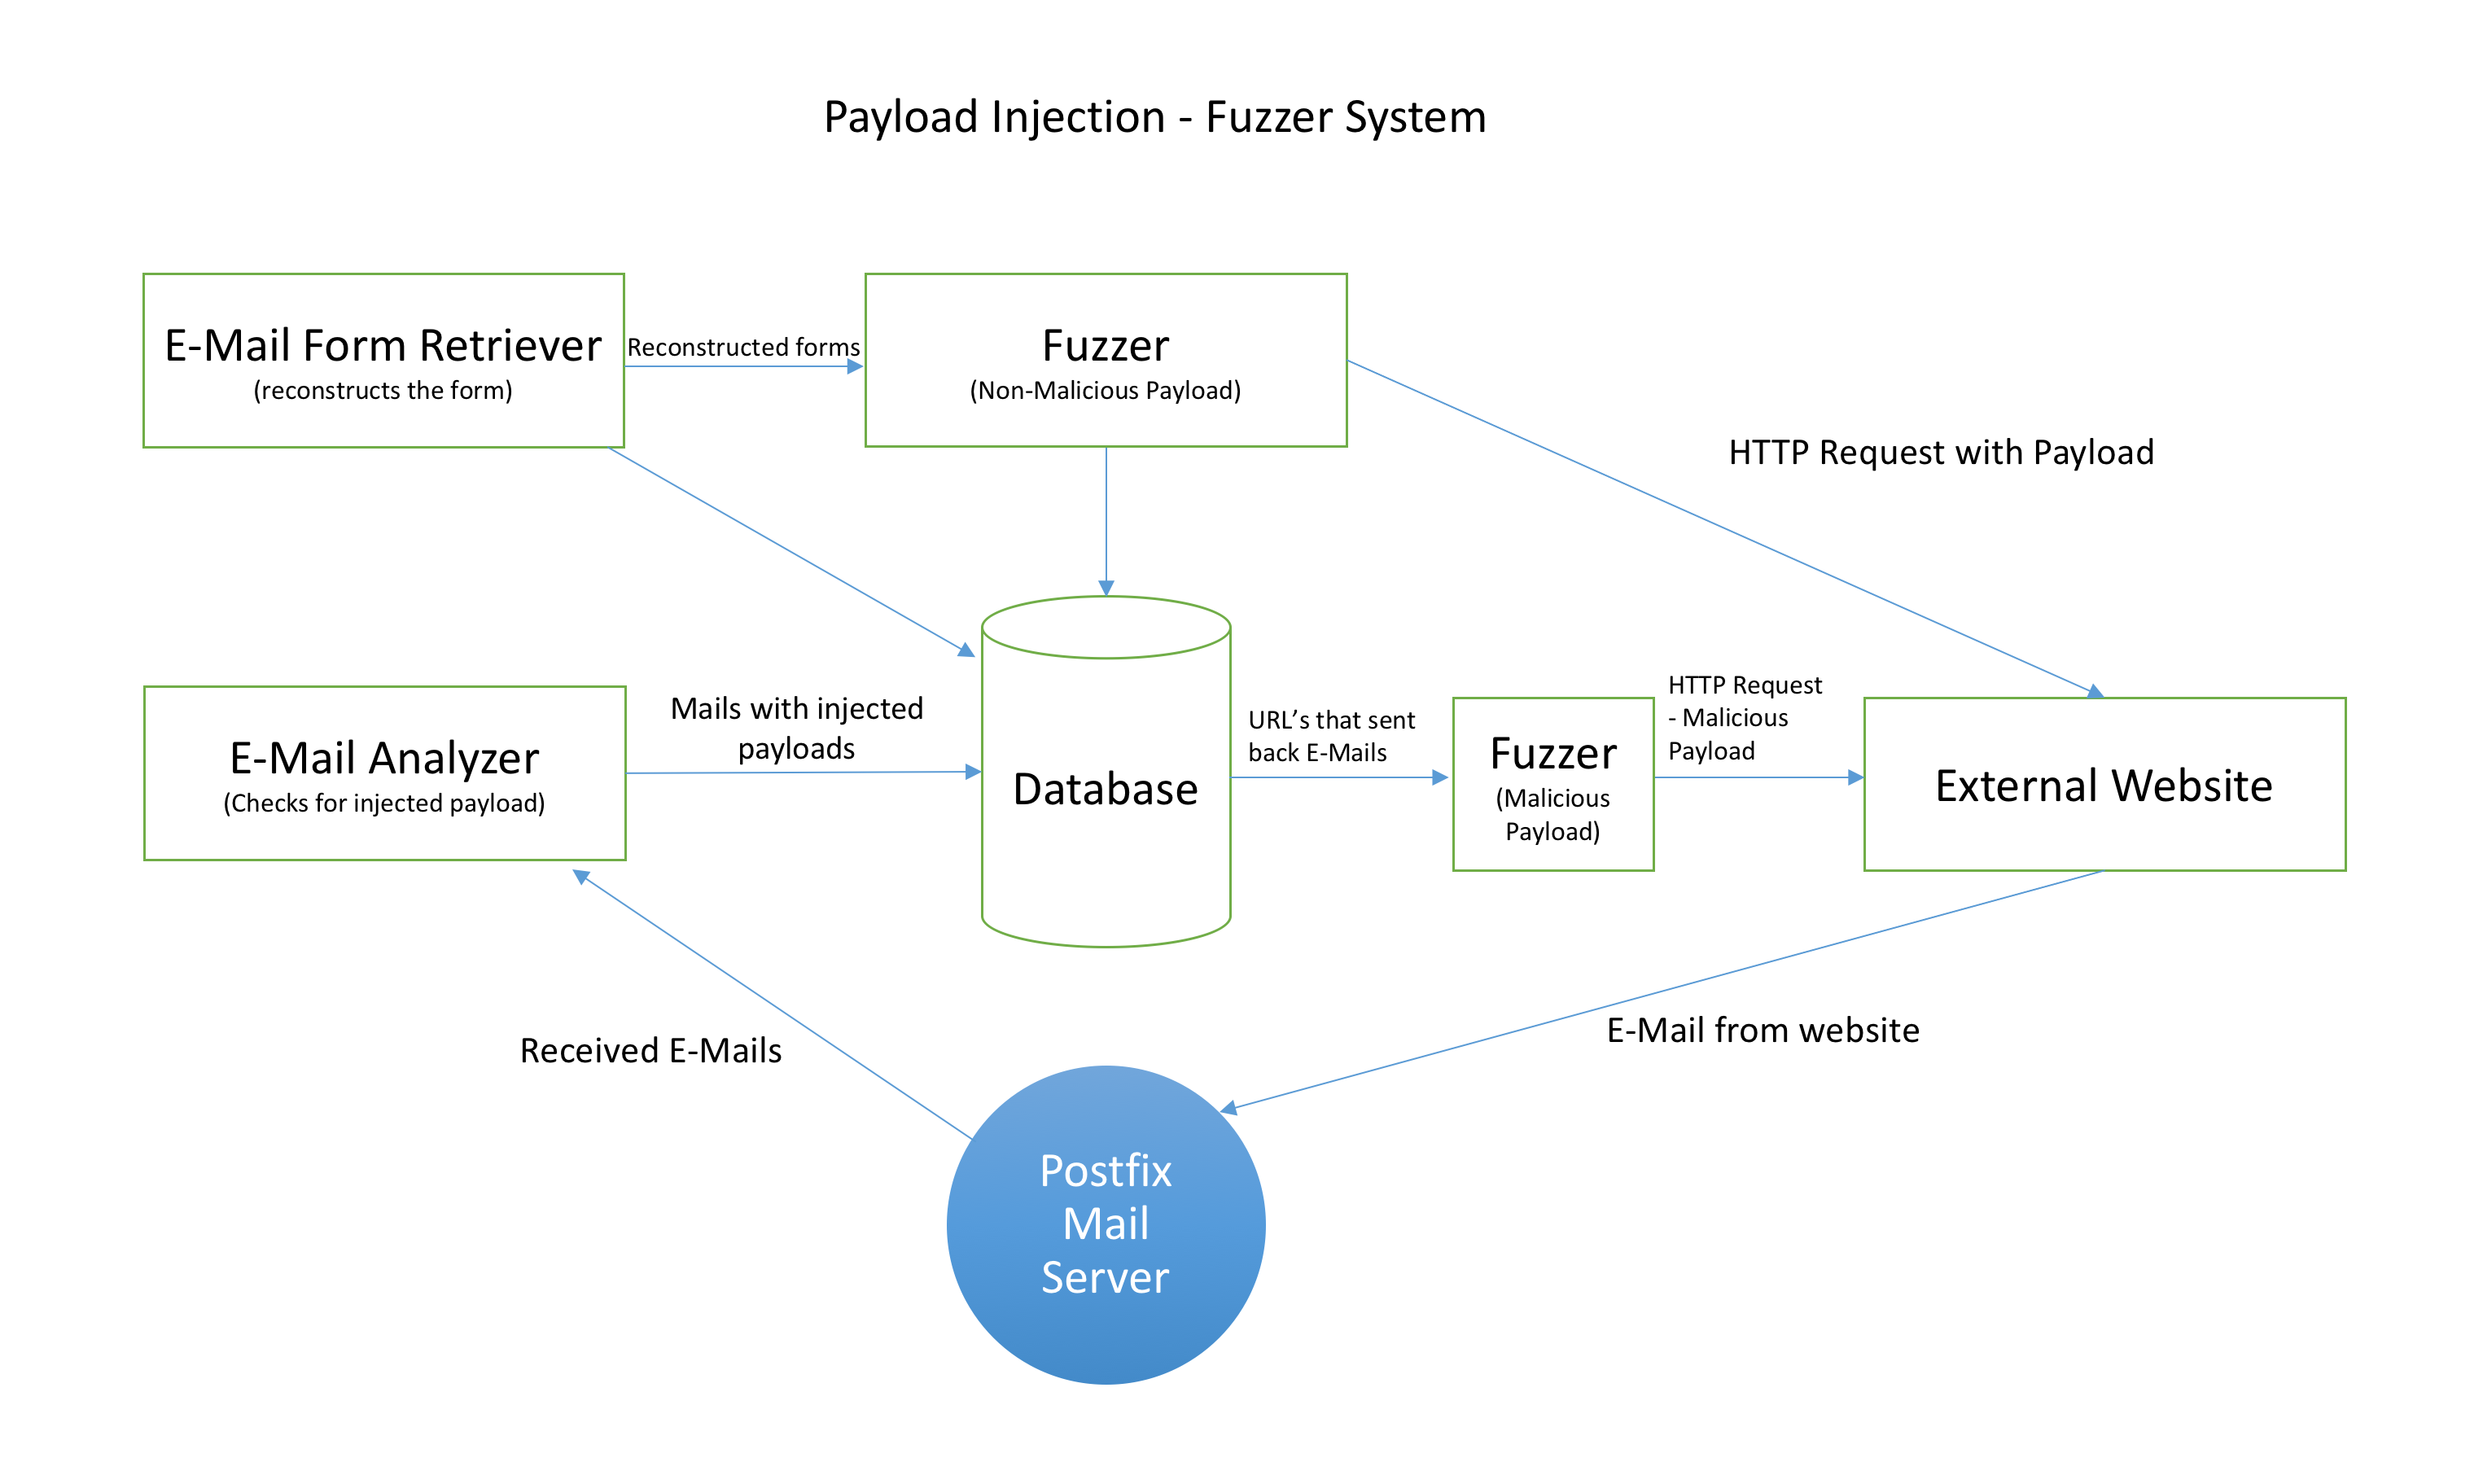
\includegraphics{System/fuzzer_design}
		\caption{A sample black and white graphic.}
	\end{figure}
	
	\begin{figure}
		\centering
		%\includegraphics[height=1in, width=1in]{fly.eps}
		\caption{A sample black and white graphic
			that has been resized with the \texttt{includegraphics} command.}
	\end{figure}
	
	
	As was the case with tables, you may want a figure
	that spans two columns.  To do this, and still to
	ensure proper ``floating'' placement of tables, use the environment
	\textbf{figure*} to enclose the figure and its caption.
	and don't forget to end the environment with
	{figure*}, not {figure}!
	
	\begin{figure*}
		\centering
		%\includegraphics{flies.eps}
		\caption{A sample black and white graphic
			that needs to span two columns of text.}
	\end{figure*}
	
	\subsection{Theorem-like Constructs}
	Other common constructs that may occur in your article are
	the forms for logical constructs like theorems, axioms,
	corollaries and proofs.  There are
	two forms, one produced by the
	command \texttt{{\char'134}newtheorem} and the
	other by the command \texttt{{\char'134}newdef}; perhaps
	the clearest and easiest way to distinguish them is
	to compare the two in the output of this sample document:
	
	This uses the \textbf{theorem} environment, created by
	the\linebreak\texttt{{\char'134}newtheorem} command:
	\newtheorem{theorem}{Theorem}
	\begin{theorem}
		Let $f$ be continuous on $[a,b]$.  If $G$ is
		an antiderivative for $f$ on $[a,b]$, then
		\begin{displaymath}\int^b_af(t)dt = G(b) - G(a).\end{displaymath}
	\end{theorem}
	
	The other uses the \textbf{definition} environment, created
	by the \texttt{{\char'134}newdef} command:
	\newdef{definition}{Definition}
	\begin{definition}
		If $z$ is irrational, then by $e^z$ we mean the
		unique number which has
		logarithm $z$: \begin{displaymath}{\log e^z = z}\end{displaymath}
	\end{definition}
	
	Two lists of constructs that use one of these
	forms is given in the
	\textit{Author's  Guidelines}.
	
	There is one other similar construct environment, which is
	already set up
	for you; i.e. you must \textit{not} use
	a \texttt{{\char'134}newdef} command to
	create it: the \textbf{proof} environment.  Here
	is a example of its use:
	\begin{proof}
		Suppose on the contrary there exists a real number $L$ such that
		\begin{displaymath}
		\lim_{x\rightarrow\infty} \frac{f(x)}{g(x)} = L.
		\end{displaymath}
		Then
		\begin{displaymath}
		l=\lim_{x\rightarrow c} f(x)
		= \lim_{x\rightarrow c}
		\left[ g{x} \cdot \frac{f(x)}{g(x)} \right ]
		= \lim_{x\rightarrow c} g(x) \cdot \lim_{x\rightarrow c}
		\frac{f(x)}{g(x)} = 0\cdot L = 0,
		\end{displaymath}
		which contradicts our assumption that $l\neq 0$.
	\end{proof}
	
	Complete rules about using these environments and using the
	two different creation commands are in the
	\textit{Author's Guide}; please consult it for more
	detailed instructions.  If you need to use another construct,
	not listed therein, which you want to have the same
	formatting as the Theorem
	or the Definition\cite{salas:calculus} shown above,
	use the \texttt{{\char'134}newtheorem} or the
	\texttt{{\char'134}newdef} command,
	respectively, to create it.
	
	\subsection*{A {\secit Caveat} for the \TeX\ Expert}
	Because you have just been given permission to
	use the \texttt{{\char'134}newdef} command to create a
	new form, you might think you can
	use \TeX's \texttt{{\char'134}def} to create a
	new command: \textit{Please refrain from doing this!}
	Remember that your \LaTeX\ source code is primarily intended
	to create camera-ready copy, but may be converted
	to other forms -- e.g. HTML. If you inadvertently omit
	some or all of the \texttt{{\char'134}def}s recompilation will
	be, to say the least, problematic.
	
	\section{Conclusions}
	This paragraph will end the body of this sample document.
	Remember that you might still have Acknowledgments or
	Appendices; brief samples of these
	follow.  There is still the Bibliography to deal with; and
	we will make a disclaimer about that here: with the exception
	of the reference to the \LaTeX\ book, the citations in
	this paper are to articles which have nothing to
	do with the present subject and are used as
	examples only.
	%\end{document}  % This is where a 'short' article might terminate
	
	%ACKNOWLEDGMENTS are optional
	\section{Acknowledgments}
	This section is optional; it is a location for you
	to acknowledge grants, funding, editing assistance and
	what have you.  In the present case, for example, the
	authors would like to thank Gerald Murray of ACM for
	his help in codifying this \textit{Author's Guide}
	and the \textbf{.cls} and \textbf{.tex} files that it describes.
	
	%
	% The following two commands are all you need in the
	% initial runs of your .tex file to
	% produce the bibliography for the citations in your paper.
	\bibliographystyle{abbrv}
	\bibliography{biblio}  % sigproc.bib is the name of the Bibliography in this case
	% You must have a proper ".bib" file
	%  and remember to run:
	% latex bibtex latex latex
	% to resolve all references
	%
	% ACM needs 'a single self-contained file'!
	%
	%APPENDICES are optional
	%\balancecolumns
	\appendix
	%Appendix A
	\section{Headings in Appendices}
	The rules about hierarchical headings discussed above for
	the body of the article are different in the appendices.
	In the \textbf{appendix} environment, the command
	\textbf{section} is used to
	indicate the start of each Appendix, with alphabetic order
	designation (i.e. the first is A, the second B, etc.) and
	a title (if you include one).  So, if you need
	hierarchical structure
	\textit{within} an Appendix, start with \textbf{subsection} as the
	highest level. Here is an outline of the body of this
	document in Appendix-appropriate form:
	\subsection{Introduction}
	\subsection{The Body of the Paper}
	\subsubsection{Type Changes and  Special Characters}
	\subsubsection{Math Equations}
	\paragraph{Inline (In-text) Equations}
	\paragraph{Display Equations}
	\subsubsection{Citations}
	\subsubsection{Tables}
	\subsubsection{Figures}
	\subsubsection{Theorem-like Constructs}
	\subsubsection*{A Caveat for the \TeX\ Expert}
	\subsection{Conclusions}
	\subsection{Acknowledgments}
	\subsection{Additional Authors}
	This section is inserted by \LaTeX; you do not insert it.
	You just add the names and information in the
	\texttt{{\char'134}additionalauthors} command at the start
	of the document.
	\subsection{References}
	Generated by bibtex from your ~.bib file.  Run latex,
	then bibtex, then latex twice (to resolve references)
	to create the ~.bbl file.  Insert that ~.bbl file into
	the .tex source file and comment out
	the command \texttt{{\char'134}thebibliography}.
	% This next section command marks the start of
	% Appendix B, and does not continue the present hierarchy
	\section{More Help for the Hardy}
	The sig-alternate.cls file itself is chock-full of succinct
	and helpful comments.  If you consider yourself a moderately
	experienced to expert user of \LaTeX, you may find reading
	it useful but please remember not to change it.
	%\balancecolumns % GM June 2007
	% That's all folks!
\end{document}
